% =====================================================================
%  neuralCSCG -- arXiv preprint
%  Two-column LaTeX article. Compiles with a standard TeX Live install:
%     pdflatex neuralCSCG_preprint.tex   (run twice for references)
%  Figures are expected in ./figures/
%  TODO: fill in author names and affiliation below.
% =====================================================================
\documentclass[twocolumn,10pt]{article}

\usepackage[a4paper,margin=0.78in]{geometry}
\usepackage{amsmath,amssymb,amsthm,mathtools}
\usepackage{graphicx}
\usepackage{booktabs}
\usepackage{array}
\usepackage{algorithm}
\usepackage{algpseudocode}
\usepackage{xcolor}
\usepackage{caption}
\usepackage{subcaption}
\usepackage{enumitem}
\usepackage{microtype}
\usepackage{tikz}
\usetikzlibrary{arrows.meta,positioning}
\usepackage[hidelinks]{hyperref}

\graphicspath{{figures/}}
\captionsetup{font=small,labelfont=bf}
\setlist{nosep,leftmargin=1.2em}

\DeclareMathOperator*{\lse}{logsumexp}
\DeclareMathOperator*{\argmax}{arg\,max}
\DeclareMathOperator*{\argmin}{arg\,min}
\newcommand{\sg}{\operatorname{sg}}
\newcommand{\R}{\mathbb{R}}
\newcommand{\Lcal}{\mathcal{L}}

\begin{document}

% ---------------------------------------------------------------------
%  Title block + full-width abstract
% ---------------------------------------------------------------------
\twocolumn[{%
  \begin{center}
    {\LARGE\bfseries Learning Cognitive Maps from Visual Experience:\\[2pt]
     A Differentiable VQ-VAE and Gradient-Trained Cloned HMM Pipeline\par}
    \vspace{1.0em}
    {\large [Author One]\quad [Author Two]\par}
    \vspace{0.35em}
    {\normalsize\itshape $^{1}$[Laboratory], [Institution], [City], [Country]\par}
    \vspace{0.35em}
    {\small Preprint. \today\par}
  \end{center}
  \vspace{0.5em}
  \begin{center}
  \begin{minipage}{0.87\textwidth}
    \small
    \noindent\textbf{Abstract.}
    Building a structured internal model of an environment from a stream of
    raw observations and actions is a core problem in both machine learning
    and the study of cognitive maps. Sequence models such as the
    Clone-Structured Cognitive Graph (CSCG) can recover environment topology,
    but they assume a \emph{discrete} observation alphabet; an agent that
    perceives pixels does not have one. We present an end-to-end pipeline that
    couples a VQ-VAE perceptual front-end to an action-conditioned cloned
    hidden Markov model (HMM) and trains the two jointly. Our key technical
    contribution is a differentiable, \emph{soft-emission} formulation of the
    cloned-HMM forward algorithm: the encoder emits a posterior over a learned
    codebook, the sequence model consumes it in log-space, and gradients from
    the topological objective propagate back into perception. We further
    introduce loss-balancing mechanisms --- length normalization, weight
    annealing, and a codebook-diversity penalty --- that make joint training
    stable. On controlled MNIST grid-world benchmarks with strong perceptual
    aliasing, the pipeline recovers the physical adjacency graph with
    \textbf{100\% edge recall}, \textbf{0.95--0.98} state-to-place purity, and
    best-threshold map F1 of \textbf{0.67--0.87} across five environments. We
    give complete formal definitions of the model, the joint objective, and
    the evaluation suite.
    \par\smallskip
    \noindent\textbf{Keywords:} cognitive maps, vector-quantized
    representation learning, cloned HMM, CSCG, differentiable sequence
    models, topology recovery.
  \end{minipage}
  \end{center}
  \vspace{1.6em}
}]

% ---------------------------------------------------------------------
\section{Introduction}
\label{sec:intro}

An agent moving through the world receives a stream of high-dimensional
sensory observations together with a record of its own actions. From this
stream alone, can it construct a \emph{cognitive map} --- a structured
internal model that recovers the relational and topological structure of the
environment~\cite{tolman1948}? This question is central both to machine
learning, where it underlies world models and navigation, and to systems
neuroscience, where the hippocampal--entorhinal system is the canonical
substrate of spatial and relational maps.

Learning such a map from raw perception is hard for three coupled reasons.
\emph{(i) Perceptual aliasing:} the same place can look different across
visits, and distinct places can look identical, so raw appearance is not a
reliable identity signal. \emph{(ii) Discretization:} sequence models that
provably recover topology --- in particular the Clone-Structured Cognitive
Graph (CSCG)~\cite{george2021}, a cloned hidden Markov model --- assume a
\emph{discrete} observation alphabet, whereas a real agent observes pixels.
\emph{(iii) Cooperation:} a perception module trained only to reconstruct
images has no incentive to produce \emph{sequence-friendly} tokens, and a
sequence model handed unstable tokens cannot recover structure.

Existing components address these difficulties only in isolation. The CSCG
recovers topology but takes the discrete alphabet as given. The
VQ-VAE~\cite{oord2017,razavi2019} learns a discrete codebook but optimizes
reconstruction alone. \textbf{No existing pipeline trains the perceptual
discretizer and the topological sequence model together so that perception
becomes sequence-aware.} Closing that gap is the subject of this paper.

\paragraph{Contributions.}
\begin{enumerate}
  \item An \textbf{end-to-end pipeline} that maps raw images to a topological
        cognitive map by coupling a VQ-VAE to an action-conditioned cloned
        HMM (Section~\ref{sec:methods}).
  \item A \textbf{differentiable, soft-emission cloned HMM}: the forward
        algorithm is implemented as a differentiable log-space computation,
        so the sequence objective can be trained by backpropagation and
        gradients reach the perceptual front-end
        (Sections~\ref{sec:cscg}--\ref{sec:soft}).
  \item \textbf{Loss-balancing for stable joint training} --- length
        normalization, weight annealing, a diversity penalty, and
        anti-collapse safeguards (Section~\ref{sec:joint}).
  \item A formal, reusable \textbf{topology-recovery evaluation suite}
        (Section~\ref{sec:metrics}).
  \item An empirical study on five MNIST grid-world environments with strong
        aliasing (Sections~\ref{sec:setup}--\ref{sec:results}).
\end{enumerate}

% ---------------------------------------------------------------------
\section{Related Work}
\label{sec:related}

\paragraph{Discrete representation learning.}
The VQ-VAE~\cite{oord2017} introduced a learned discrete bottleneck trained
with a straight-through estimator~\cite{bengio2013} and a commitment loss;
\cite{razavi2019} stabilized the codebook with exponential-moving-average
(EMA) updates. These models optimize reconstruction; they are not trained for
downstream sequential structure, which is the coupling we add.

\paragraph{Cloned HMMs and cognitive maps.}
The CSCG~\cite{george2021} is an action-augmented cloned HMM in which each
observation symbol owns several latent ``clones''; clones with identical
emissions but different transition contexts disambiguate perceptual aliasing
and yield interpretable maps. Cloned HMMs are classically trained by
Expectation--Maximization. The Tolman--Eichenbaum Machine~\cite{whittington2020}
is a related neural account of relational memory. We retain the CSCG model
class but make its training \emph{gradient-based}, which is what allows it to
be composed with a neural front-end.

\paragraph{HMM inference.}
The forward and Viterbi algorithms~\cite{rabiner1989} underlie our likelihood
and decoding; our contribution is to express the forward recursion as a
differentiable log-space graph and to admit \emph{soft} emissions so that the
likelihood is differentiable in the encoder output.

% ---------------------------------------------------------------------
\section{Materials and Methods}
\label{sec:methods}

\subsection{Problem formulation}
\label{sec:problem}

An agent produces an episode of length $T$: observations
$x_{1:T}$ with $x_t\in\mathcal{X}\subset\R^{H\times W\times C}$ and actions
$a_{1:T-1}$ with $a_t\in\mathcal{A}=\{1,\dots,A\}$, where $a_t$ is taken
between times $t$ and $t{+}1$. Each observation is emitted at an
underlying physical place $g_t\in\mathcal{G}$; the environment has a true
undirected adjacency graph $\mathcal{M}=(\mathcal{G},\mathcal{E})$. The places
$g_t$ and edges $\mathcal{E}$ are used \emph{only for evaluation} and are
never seen during training. The goal is to learn, from $(x_{1:T},a_{1:T-1})$
alone, a latent model whose transition structure recovers $\mathcal{M}$.

The pipeline (Fig.~\ref{fig:pipeline}) has two modules: a VQ-VAE that maps
each image to a discrete token, and an action-conditioned cloned HMM over
those tokens whose latent graph is the learned map.

\begin{figure*}[t]
\centering
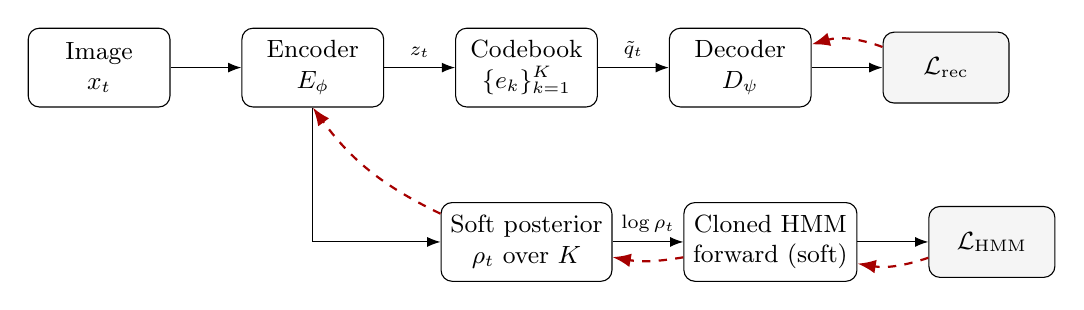
\begin{tikzpicture}[
  >=Latex, node distance=8mm and 9mm,
  box/.style={draw, rounded corners, minimum height=10mm, minimum width=18mm,
              align=center, font=\small},
  loss/.style={draw, rounded corners, minimum height=9mm, minimum width=16mm,
               align=center, font=\small\itshape, fill=black!4},
  grad/.style={->, dashed, red!65!black, thick}
]
\node[box] (img)  {Image\\$x_t$};
\node[box, right=of img] (enc)  {Encoder\\$E_\phi$};
\node[box, right=of enc] (vq)   {Codebook\\$\{e_k\}_{k=1}^{K}$};
\node[box, right=of vq]  (dec)  {Decoder\\$D_\psi$};
\node[loss, right=of dec] (rec) {$\Lcal_{\mathrm{rec}}$};
\node[box, below=12mm of vq] (soft) {Soft posterior\\$\rho_t$ over $K$};
\node[box, right=of soft] (hmm) {Cloned HMM\\forward (soft)};
\node[loss, right=of hmm] (nll) {$\Lcal_{\mathrm{HMM}}$};
\draw[->] (img)--(enc);
\draw[->] (enc)--node[above,font=\scriptsize]{$z_t$}(vq);
\draw[->] (vq)--node[above,font=\scriptsize]{$\tilde q_t$}(dec);
\draw[->] (dec)--(rec);
\draw[->] (enc.south) |- (soft);
\draw[->] (soft)--node[above,font=\scriptsize]{$\log\rho_t$}(hmm);
\draw[->] (hmm)--(nll);
\draw[grad] (rec) to[bend right=18] (dec);
\draw[grad] (nll) to[bend left=14] (hmm);
\draw[grad] (hmm) to[bend left=10] (soft);
\draw[grad] (soft) to[bend left=14] (enc.south);
\end{tikzpicture}
\caption{\textbf{The neuralCSCG pipeline.} Solid arrows: forward computation.
Dashed red arrows: gradient flow. The encoder feeds both a reconstruction
branch (hard quantization $\tilde q_t$ + decoder) and a sequence branch (soft
codebook posterior $\rho_t$ + differentiable cloned-HMM forward pass). Because
the HMM likelihood is differentiable in $\rho_t$, the topological objective
$\Lcal_{\mathrm{HMM}}$ shapes the encoder. The codebook itself is updated by
EMA, not by gradients.}
\label{fig:pipeline}
\end{figure*}

\subsection{Perceptual front-end: VQ-VAE}
\label{sec:vqvae}

\paragraph{Encoder and quantization.}
A convolutional encoder $E_\phi:\mathcal{X}\to\R^{D}$ maps each image to a
latent $z_t=E_\phi(x_t)$. A codebook $\{e_k\}_{k=1}^{K}$, $e_k\in\R^{D}$,
defines a discrete token by nearest-neighbour assignment,
\begin{equation}
k_t=\argmin_{k\in\{1,\dots,K\}}\;\lVert z_t-e_k\rVert_2^2 ,
\qquad q_t=e_{k_t},
\label{eq:quantize}
\end{equation}
where the squared distance is computed as
$\lVert z-e_k\rVert_2^2=\lVert z\rVert_2^2-2\langle z,e_k\rangle+\lVert
e_k\rVert_2^2$. Gradients cross the non-differentiable $\argmin$ by the
straight-through estimator~\cite{bengio2013},
\begin{equation}
\tilde q_t = z_t + \sg(q_t-z_t),
\label{eq:ste}
\end{equation}
where $\sg(\cdot)$ is the stop-gradient operator, so the forward value is
$q_t$ while $\partial\tilde q_t/\partial z_t=I$. A decoder $D_\psi$
reconstructs $\hat x_t=D_\psi(\tilde q_t)$.

\paragraph{Losses.}
Over a minibatch $\mathcal{B}$,
\begin{align}
\Lcal_{\mathrm{rec}} &= \tfrac{1}{|\mathcal{B}|}\textstyle\sum_{t}
   \lVert x_t-\hat x_t\rVert_2^2 ,\\
\Lcal_{\mathrm{commit}} &= \tfrac{1}{|\mathcal{B}|}\textstyle\sum_{t}
   \lVert \sg(q_t)-z_t\rVert_2^2 ,
\label{eq:vqlosses}
\end{align}
the second term pulling encoder outputs toward their assigned code.

\paragraph{EMA codebook updates.}
The codebook is \emph{not} trained by gradient descent. With decay
$\gamma\in(0,1)$, per batch we accumulate, for every code $k$, a cluster size
$n_k$ and a vector sum $m_k$,
\begin{align}
n_k &\leftarrow \gamma\,n_k+(1-\gamma)\!\textstyle\sum_{t}\mathbb{1}[k_t=k],\\
m_k &\leftarrow \gamma\,m_k+(1-\gamma)\!\textstyle\sum_{t}\mathbb{1}[k_t=k]\,z_t,
\end{align}
and set $e_k\leftarrow m_k/\hat n_k$ with Laplace-smoothed size
\begin{equation}
\hat n_k=\frac{n_k+\epsilon}{\bigl(\sum_{k'}n_{k'}\bigr)+K\epsilon}
        \;\Bigl(\textstyle\sum_{k'}n_{k'}\Bigr).
\end{equation}

\paragraph{Soft codebook posterior.}
For the differentiable coupling (Section~\ref{sec:soft}) the encoder also
emits a temperature-controlled posterior over the codebook,
\begin{equation}
\log\rho_t(k) = \log\operatorname{softmax}_{k}
   \!\Bigl(-\lVert z_t-e_k\rVert_2^2/\tau\Bigr),
\label{eq:soft}
\end{equation}
which is differentiable in $z_t$. As $\tau\to0$, $\rho_t$ concentrates on
$k_t$ and~\eqref{eq:soft} recovers the hard assignment~\eqref{eq:quantize}.

\subsection{Sequence model: action-conditioned cloned HMM}
\label{sec:cscg}

\paragraph{State space and clone structure.}
Each token $k$ is assigned $C_k\ge1$ \emph{clones} --- latent states that all
emit token $k$ but participate in different transition contexts. With a
trailing \emph{sink} state $\bot$, the state space is
$\mathcal{S}=\{1,\dots,N\}$ with $N=1+\sum_{k=1}^{K}C_k$. A fixed map
$\omega:\mathcal{S}\!\setminus\!\{\bot\}\to\{1,\dots,K\}$ gives the token each
state emits; in the uniform case $C_k\equiv C$ and
$\omega(s)=\lceil s/C\rceil$. Emissions are \emph{deterministic}:
\begin{equation}
B_{s,o}=\mathbb{1}[\omega(s)=o],\qquad
\log B_{s,o}=\begin{cases}0,&\omega(s)=o\\-\infty,&\text{otherwise,}\end{cases}
\end{equation}
and the sink emits no real token. Clones are exactly the mechanism that
disambiguates aliasing: one token observed at two places is explained by two
clones with distinct transition rows.

\paragraph{Parameters.}
The model has initial-state logits $\pi\in\R^{N}$ and action-conditioned
transition logits $\Theta\in\R^{A\times N\times N}$, yielding
\begin{equation}
\bar\pi=\operatorname{softmax}(\pi),\qquad
T_{a,i,j}=\operatorname{softmax}_{j}\bigl(\Theta_{a,i,\cdot}\bigr).
\end{equation}
All learning resides in $(\pi,\Theta)$; emissions are fixed.

\paragraph{Forward likelihood.}
Writing $\lse_i u_i=\log\sum_i e^{u_i}$, the log-forward messages for an
episode $(o_{1:T},a_{1:T-1})$ obey
\begin{align}
\log\alpha_1(j) ={}& \log\bar\pi_j+\log B_{j,o_1},\\
\log\alpha_{t+1}(j) ={}& \lse_{i}\!\bigl[\log\alpha_t(i)+\log T_{a_t,i,j}\bigr]
                       \notag\\
   &{}+ \log B_{j,o_{t+1}},
\label{eq:forward}
\end{align}
and the episode log-likelihood is
$\ell(o_{1:T}\!\mid a_{1:T-1})=\lse_{j}\log\alpha_T(j)$. The training loss is
the mean negative log-likelihood (NLL)
\begin{equation}
\Lcal_{\mathrm{HMM}}=-\tfrac{1}{|\mathcal{B}|}
  \textstyle\sum_{(o,a)\in\mathcal{B}}\ell(o_{1:T}\mid a_{1:T-1}).
\label{eq:hmmloss}
\end{equation}

\subsection{Gradient-based training of the cloned HMM}
\label{sec:grad}

Unlike the classical EM training of cloned HMMs, we evaluate
\eqref{eq:forward}--\eqref{eq:hmmloss} as a single differentiable, log-space
computational graph (a masked time recursion over padded minibatches) and
optimize $(\pi,\Theta)$ directly by stochastic gradient descent with
Adam~\cite{kingma2015}. Log-space arithmetic with $\lse$ keeps the recursion
numerically stable over long episodes. This gradient formulation is what makes
the sequence model composable with a neural front-end.

\subsection{Differentiable soft-emission coupling}
\label{sec:soft}

To let the topological objective shape perception, we replace the hard
emission term $\log B_{j,o_{t}}$ in~\eqref{eq:forward} by the soft
log-posterior~\eqref{eq:soft} of the token that state $j$ emits:
\begin{align}
\log\alpha^{s}_1(j) ={}& \log\bar\pi_j+\log\rho_1\!\bigl(\omega(j)\bigr),\\
\log\alpha^{s}_{t+1}(j) ={}& \lse_{i}\!\bigl[\log\alpha^{s}_t(i)+\log T_{a_t,i,j}\bigr]
   \notag\\
   &{}+ \log\rho_{t+1}\!\bigl(\omega(j)\bigr),
\label{eq:softforward}
\end{align}
with the sink assigned $\log\rho_t(\bot)=-\infty$. The resulting
log-likelihood $\ell^{s}$ is differentiable in $\rho_{1:T}$ and hence,
through~\eqref{eq:soft}, in the encoder parameters $\phi$. Two properties hold
by construction:

\begin{enumerate}
\item \textbf{Consistency.} If $\rho_t$ is the one-hot distribution on the
      observed token $o_t$, then $\log\rho_t(\omega(j))=\log B_{j,o_t}$ and
      \eqref{eq:softforward} reduces exactly to the hard
      forward pass~\eqref{eq:forward}. As $\tau\to0$ the soft pipeline thus
      recovers the hard pipeline.
\item \textbf{End-to-end differentiability.} Gradients of $\Lcal_{\mathrm{HMM}}$
      propagate $\ell^{s}\!\to\!\rho\!\to\!z\!\to\!\phi$, so the encoder is
      trained, in part, to produce tokens that make the action-conditioned
      sequence \emph{explainable}.
\end{enumerate}

\subsection{Joint objective and loss balancing}
\label{sec:joint}

\paragraph{Training regimes.}
We use a deliberate progression. \emph{Phase~1 (stagewise)} trains the VQ-VAE
alone, then trains the HMM on hard tokens. \emph{Phase~2 (joint)} optimizes
encoder, decoder and $(\pi,\Theta)$ together under a combined objective.
\emph{Phase~2.5} adds loss-balancing terms that make Phase~2 stable.

\paragraph{Combined objective.}
At joint step $t$,
\begin{equation}
\Lcal_{\mathrm{joint}} = \Lcal_{\mathrm{rec}}
  + \beta\,\Lcal_{\mathrm{commit}}
  + \lambda_t\,\widetilde{\Lcal}_{\mathrm{HMM}}
  + \alpha_{\mathrm{div}}\,\Lcal_{\mathrm{div}}.
\label{eq:joint}
\end{equation}

\paragraph{Length normalization.}
The raw NLL~\eqref{eq:hmmloss} grows as $O(T)$, which on long episodes dwarfs
the $O(1)$ reconstruction term and collapses the codebook. We therefore use
the per-step NLL
\begin{equation}
\widetilde{\Lcal}_{\mathrm{HMM}}=-\tfrac{1}{|\mathcal{B}|}
   \textstyle\sum \tfrac{1}{T}\,\ell^{s}(o_{1:T}\mid a_{1:T-1}).
\end{equation}

\paragraph{Weight annealing.}
The sequence-loss weight is ramped linearly so the codebook stabilizes under
reconstruction before topological pressure turns on:
\begin{equation}
\lambda_t=\lambda\cdot\min\!\bigl(1,\;t/T_{\mathrm{anneal}}\bigr).
\end{equation}

\paragraph{Diversity penalty.}
Let $\bar\rho(k)=\frac{1}{|\mathcal{B}|}\sum_t\rho_t(k)$ be mean codebook
usage and $H(\bar\rho)=-\sum_k\bar\rho(k)\log\bar\rho(k)$ its entropy. The
penalty
\begin{equation}
\Lcal_{\mathrm{div}}=\log K-H(\bar\rho)\;\ge\;0
\end{equation}
vanishes only at uniform usage and counteracts codebook collapse.

\paragraph{Anti-collapse safeguards and finalization.}
During Phase~2 we monitor codebook perplexity and keep the
highest-perplexity checkpoint; optional $\lambda$-throttling, rollback, and
dead-code revival provide further protection. A short \emph{finalization}
phase then freezes the encoder and refines $(\pi,\Theta)$ on hard tokens with
the unnormalized loss~\eqref{eq:hmmloss}, optionally with a transition-entropy
regularizer $-\eta\sum_{a,i}H(T_{a,i,\cdot})$ to sharpen transition rows.
Algorithm~\ref{alg:joint} summarizes one joint step.

\begin{algorithm}[t]
\caption{One joint training step}
\label{alg:joint}
\begin{algorithmic}[1]
\Require image chunk $x_{1:T}$, actions $a_{1:T-1}$, weights
         $\beta,\lambda_t,\alpha_{\mathrm{div}}$, temperature $\tau$
\State $z_t \gets E_\phi(x_t)$ \Comment{encode}
\State $q_t,\tilde q_t \gets$ quantize$(z_t)$; update codebook by EMA
\State $\hat x_t \gets D_\psi(\tilde q_t)$;\;
       $\Lcal_{\mathrm{rec}},\Lcal_{\mathrm{commit}}\gets$ Eq.~(3)--(4)
\State $\log\rho_t \gets \log\operatorname{softmax}(-\lVert z_t-e_\cdot
       \rVert^2/\tau)$
\State $\ell^{s}\gets$ soft forward pass, Eq.~(12)--(13)
\State $\widetilde{\Lcal}_{\mathrm{HMM}}\gets -\ell^{s}/T$;\;
       $\Lcal_{\mathrm{div}}\gets \log K-H(\bar\rho)$
\State $\Lcal_{\mathrm{joint}}\gets$ Eq.~(11)
\State update $(\phi,\psi,\pi,\Theta)$ with Adam on
       $\nabla\Lcal_{\mathrm{joint}}$
\end{algorithmic}
\end{algorithm}

\subsection{Decoding}
\label{sec:decode}

The maximum-a-posteriori state path is obtained by the Viterbi
recursion~\cite{rabiner1989}:
\begin{align}
\delta_1(j) &= \log\bar\pi_j+\log B_{j,o_1},\\
\delta_{t+1}(j) &= \max_{i}\bigl[\delta_t(i)+\log T_{a_t,i,j}\bigr]
                   + \log B_{j,o_{t+1}},
\end{align}
with backpointers $\psi_{t+1}(j)=\argmax_i[\delta_t(i)+\log T_{a_t,i,j}]$ and
traceback $s^\star_T=\argmax_j\delta_T(j)$,
$s^\star_t=\psi_{t+1}(s^\star_{t+1})$. The decoded path $s^\star_{1:T}$ is the
basis of all evaluation.

\subsection{Token compaction and clone allocation}
In Phase~1, codes never emitted by the trained encoder are pruned and the
alphabet is relabelled to the active set. Clone counts $C_k$ may be uniform or
allocated per token (\emph{dynamic clone allocation}); the deterministic
emission structure of Section~\ref{sec:cscg} is unchanged.

\subsection{Evaluation metrics}
\label{sec:metrics}

All metrics are computed from the decoded path $s^\star_{1:T}$ of a held-out
episode together with the ground-truth places $g_{1:T}$ and edges
$\mathcal{E}$ (used only here, never in training). Let $\mathcal{V}$ be the
set of visited states and $n(s,g)=\#\{t:s^\star_t=s,\;g_t=g\}$.

\paragraph{State-to-place assignment.}
Each visited state is mapped to its majority place,
$\chi(s)=\argmax_{g}n(s,g)$.

\paragraph{Clone purity.}
\begin{equation}
\mathrm{Purity}=\frac{1}{|\mathcal{V}|}\sum_{s\in\mathcal{V}}
   \frac{\max_g n(s,g)}{\sum_g n(s,g)},
\end{equation}
with the visit-weighted variant
$\sum_s\max_g n(s,g)\,/\,T$. High purity means clone states correspond
cleanly to single physical places.

\paragraph{Projected map and edge F1.}
Latent transitions are projected onto a place graph by
\begin{equation}
W(g,g')=\max_{a}\;\max_{\substack{i,j\in\mathcal{V}\\ \chi(i)=g,\;\chi(j)=g'}}
   T_{a,i,j},
\end{equation}
and thresholded into a learned edge set
$\widehat{\mathcal{E}}(\eta)=\{(g,g'):g\neq g',\,W(g,g')>\eta\}$. With
$\mathrm{tp}=|\widehat{\mathcal{E}}\cap\mathcal{E}|$, precision, recall and
F1 are defined in the usual way. We report F1 over a threshold sweep
$\eta\in\{0.01,0.05,0.1,0.2,0.3\}$.

\paragraph{Action-next-cell accuracy.}
For every represented place $g$ and action $a$, the predicted next place
$\argmax_{g'}W_a(g,g')$ is compared with the environment's true successor
$\mathrm{next}(g,a)$.

\paragraph{Token--place entropies.}
From the empirical token/place co-occurrence we report $H(\text{token}\mid
\text{place})$ and $H(\text{place}\mid\text{token})$; the former is small when
perception is consistent, the latter reflects the (irreducible) aliasing of
the environment.

\subsection{Implementation and hyperparameters}
\label{sec:impl}

The encoder is three convolutional layers (strides $2,2,1$) followed by global
average pooling and a dense projection to $\R^{D}$; the decoder mirrors it. The
HMM forward pass, soft forward pass and training steps are implemented as
compiled TensorFlow graphs; Viterbi decoding is eager. Transition logits are
initialized with a bias toward the sink state so probability mass is
well-defined before training. Table~\ref{tab:hyper} lists all hyperparameters.

\begin{table}[t]
\centering
\caption{Hyperparameters. Ranges span the five environments of
Section~\ref{sec:setup}.}
\label{tab:hyper}
\small
\begin{tabular}{@{}lll@{}}
\toprule
\textbf{Component / parameter} & \textbf{Symbol} & \textbf{Value} \\
\midrule
\multicolumn{3}{@{}l}{\emph{VQ-VAE}}\\
Codebook size            & $K$        & $4$--$10$ \\
Embedding dimension      & $D$        & $32$ \\
Encoder base width       & ---        & $32$ \\
Commitment weight        & $\beta$    & $0.25$ \\
EMA decay                & $\gamma$   & $0.99$ \\
EMA smoothing            & $\epsilon$ & $10^{-5}$ \\
\midrule
\multicolumn{3}{@{}l}{\emph{Cloned HMM / CSCG}}\\
Action alphabet          & $A$        & $4$ \\
Clones per token         & $C_k$      & $5$--$20$ \\
Latent states            & $N$        & $21$--$201$ \\
\midrule
\multicolumn{3}{@{}l}{\emph{Joint training (Phase 2 / 2.5)}}\\
Softmax temperature      & $\tau$     & $1.0$ \\
HMM-loss weight          & $\lambda$  & $1.0$ \\
Anneal horizon           & $T_{\mathrm{anneal}}$ & iters$/4$ \\
Diversity weight         & $\alpha_{\mathrm{div}}$ & $0.1$ \\
HMM learning-rate factor & ---        & $100$ \\
Chunk length             & $T$        & $256$ \\
Joint minibatch          & $|\mathcal{B}|$ & $4$ \\
Joint iterations         & ---        & $2000$--$5000$ \\
\midrule
\multicolumn{3}{@{}l}{\emph{Finalization}}\\
Iterations               & ---        & $1000$--$5000$ \\
Transition-entropy weight& $\eta$     & $10^{-3}$ \\
Minibatch                & ---        & $8$ \\
\midrule
\multicolumn{3}{@{}l}{\emph{Optimization and data}}\\
Optimizer                & ---        & Adam~\cite{kingma2015} \\
VQ-VAE / joint learning rate & ---    & $3\times10^{-4}$ \\
Finalization learning rate   & ---    & $10^{-2}$ \\
Episodes $\times$ steps  & ---        & $(4\text{--}10)\times10{,}000$ \\
\bottomrule
\end{tabular}
\end{table}

% ---------------------------------------------------------------------
\section{Experimental Setup}
\label{sec:setup}

\subsection{The MNIST grid-world benchmark}
The benchmark is a 2-D grid in which every cell carries a digit class.
\emph{Visiting a cell returns a randomly drawn MNIST image~\cite{lecun1998} of
that digit}, so the same place never looks identical twice and cells sharing a
digit are perceptually aliased. The agent has four actions (up, down, left,
right) with sticky walls. Ground-truth topology is known exactly, which makes
the benchmark a controlled testbed for topology recovery.

\subsection{Environments}
We study five environments of increasing difficulty
(Table~\ref{tab:envs}): \texttt{aliased}, a $4\times4$ grid in which four
digits each recur four times; \texttt{corridors}, a $5\times5$ grid with walls
and repeated digits; two $6\times6$ rooms differing in clone allocation; and
\texttt{two\_rooms}, a $13\times9$ map of two offset, interconnected rooms ---
the largest and most aliased case. Figure~\ref{fig:env} shows
\texttt{two\_rooms} rendered with one MNIST sample per cell.

\begin{table}[t]
\centering
\caption{Benchmark environments.}
\label{tab:envs}
\small
\begin{tabular}{@{}llcc@{}}
\toprule
\textbf{Environment} & \textbf{Grid} & \textbf{Tokens $K$} & \textbf{States $N$}\\
\midrule
\texttt{aliased}            & $4\times4$  & $4$  & $21$ \\
\texttt{corridors}          & $5\times5$  & $6$  & $31$ \\
\texttt{room} (uniform)     & $6\times6$  & $10$ & $201$ \\
\texttt{room} (dynamic)     & $6\times6$  & $10$ & $57$ \\
\texttt{two\_rooms}         & $13\times9$ & $10$ & $151$ \\
\bottomrule
\end{tabular}
\end{table}

\begin{figure}[t]
\centering
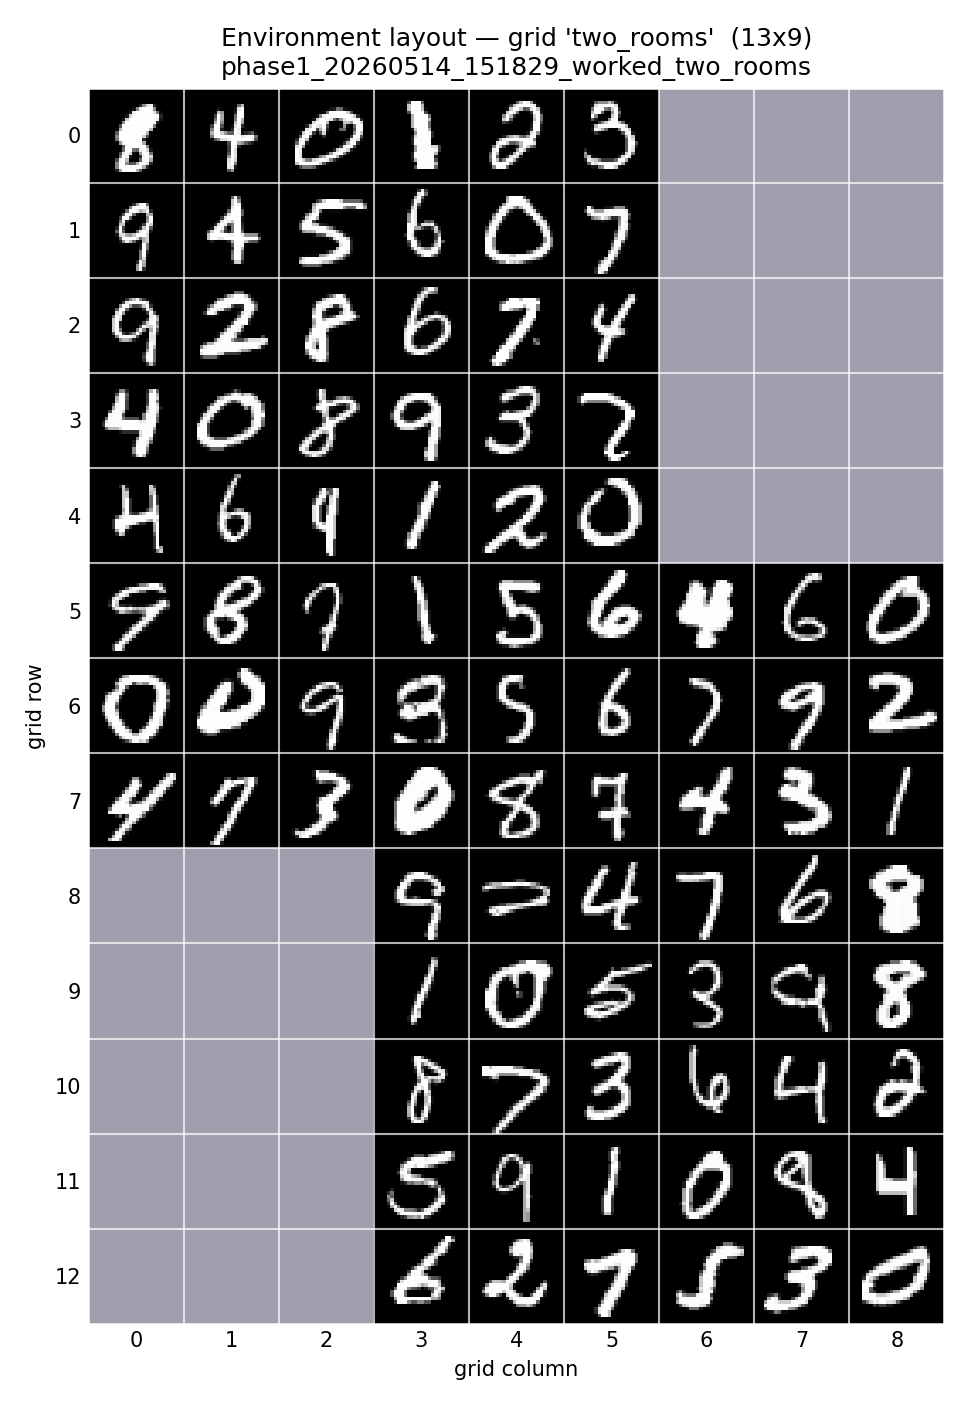
\includegraphics[width=0.74\columnwidth,height=0.42\textheight,%
keepaspectratio]{environment.png}
\caption{The \texttt{two\_rooms} environment, each cell shown as one MNIST
sample of its digit. Cells that share a digit are perceptually aliased; the
two rooms overlap through a shared corner.}
\label{fig:env}
\end{figure}

\subsection{Protocol}
Trajectories are action-conditioned random walks ($4$--$10$ episodes of
$10{,}000$ steps). Each run executes VQ-VAE warmup, joint training
(Phase~2/2.5) and finalization, then is evaluated on a held-out episode with
the metrics of Section~\ref{sec:metrics}. An optional, benchmark-only auxiliary
digit-classification loss may be used during VQ-VAE warmup; it is disableable,
since in a general environment object classes are unknown.

% ---------------------------------------------------------------------
\section{Results}
\label{sec:results}

\subsection{Perceptual discretization}
The VQ-VAE produces a clean, near-deterministic discretization. Across
environments, mean tokens per cell is $1.0$--$1.2$ and the conditional entropy
$H(\text{token}\mid\text{place})$ is $0.09$--$0.23$ nats: a place almost
always emits a single token despite never being seen twice
(Fig.~\ref{fig:tokencell}). Codebook perplexity tracks the number of digit
classes (Fig.~\ref{fig:codebook}), and reconstructions remain faithful
(Fig.~\ref{fig:recon}), confirming that the codebook does not collapse under
the joint objective.

\begin{figure}[t]
\centering
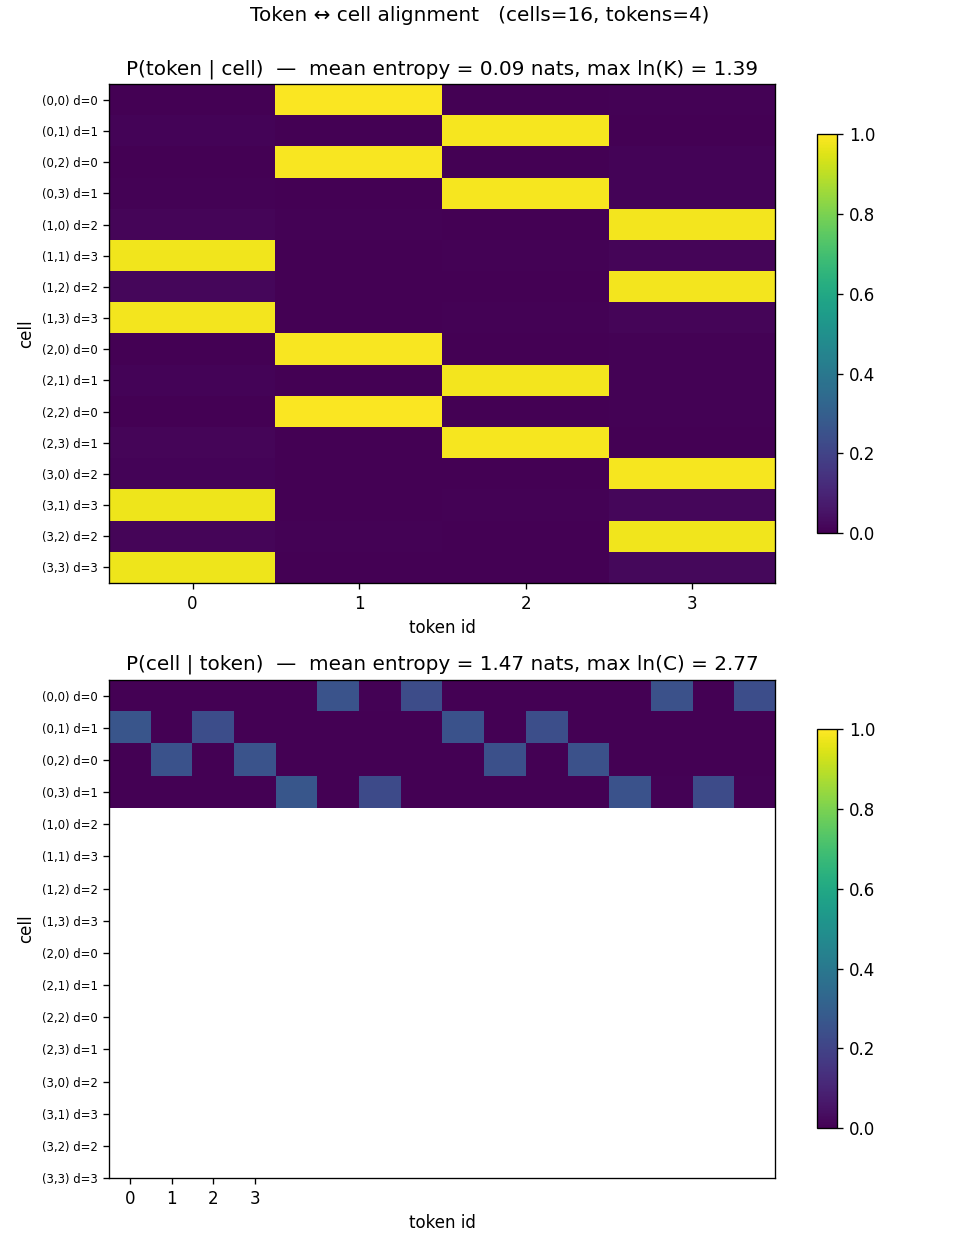
\includegraphics[width=0.92\columnwidth,height=0.42\textheight,%
keepaspectratio]{token_cell_heatmap.png}
\caption{Token$\leftrightarrow$place alignment, shown for the
\texttt{aliased} environment as a clear illustration; the pattern is
representative of all environments. Top: $P(\text{token}\mid\text{place})$
--- one bright entry per row (one token per place). Bottom:
$P(\text{place}\mid\text{token})$ --- each token spreads over the four
aliased cells that share its digit, the environment's intrinsic aliasing.}
\label{fig:tokencell}
\end{figure}

\begin{figure}[t]
\centering
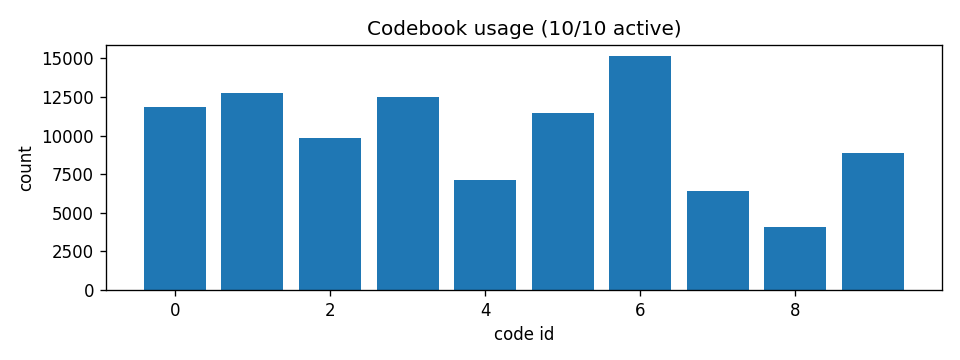
\includegraphics[width=0.95\columnwidth]{codebook_usage.png}
\caption{Codebook utilization for \texttt{two\_rooms}: all codes remain
active; perplexity does not collapse during joint training.}
\label{fig:codebook}
\end{figure}

\begin{figure*}[t]
\centering
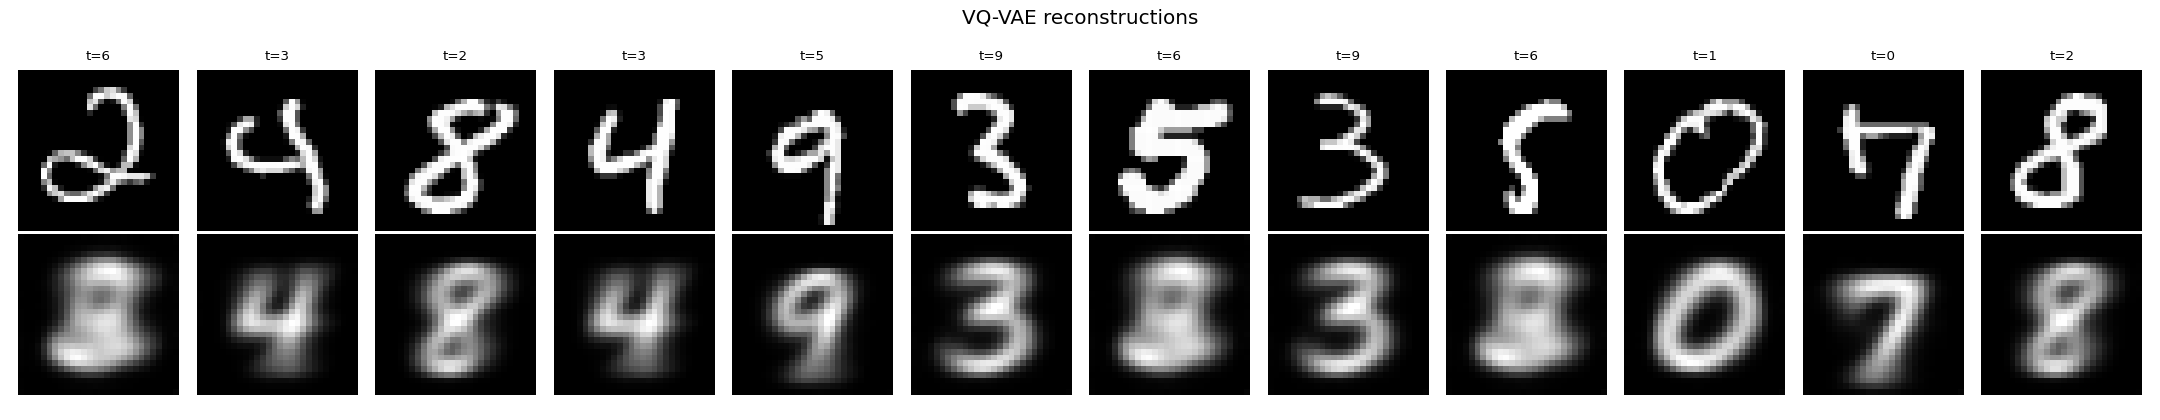
\includegraphics[width=0.92\textwidth]{reconstructions.png}
\caption{Inputs (top) and VQ-VAE reconstructions (bottom) with the assigned
token id. Reconstruction stays meaningful throughout joint training.}
\label{fig:recon}
\end{figure*}

\subsection{Clone-state purity}
Decoded clone states map cleanly to physical places. The visit-weighted
state-to-place purity is $0.95$--$0.98$ across the four fully scored
environments (Table~\ref{tab:results}), and every visited place is represented
by at least one clone. The decoded clone graph (Fig.~\ref{fig:viterbi})
exposes the recovered topology directly: nodes are clone states drawn as the
MNIST digit they represent, and edges are the action-conditioned transitions
actually taken.

\begin{figure}[t]
\centering

\includegraphics[width=0.97\columnwidth,height=0.44\textheight,%
keepaspectratio]{viterbi_graph.png}
\caption{Decoded clone-state graph for \texttt{two\_rooms}; each node is drawn
as an MNIST sample of the digit it represents, edges are Viterbi-path
transitions. The two-room layout is visible in the latent graph.}
\label{fig:viterbi}
\end{figure}

\subsection{Topological map recovery}
The central result is that the learned latent graph \emph{contains} the true
environment graph. Map-edge \textbf{recall is $1.00$ in every scored run} ---
no physical adjacency is missed. The open difficulty is precision: at a low
threshold the projected graph also includes many weak false edges. A threshold
sweep makes the trade-off explicit (Table~\ref{tab:sweep}): on
\texttt{corridors}, precision rises from $0.24$ at $\eta=0.01$ to $0.77$ at
$\eta=0.3$ while recall stays at $1.00$, lifting F1 to $0.87$. The
best-threshold F1 is $0.67$--$0.87$ across environments
(Table~\ref{tab:results}). Figure~\ref{fig:projected} shows the projected map
for \texttt{two\_rooms}: every true edge (green) is recovered and the false
edges (red) are the residual weak transitions.

\begin{table}[t]
\centering
\caption{Edge-threshold sweep on \texttt{corridors}. Recall is $1.00$
throughout; precision and F1 increase with the threshold $\eta$.}
\label{tab:sweep}
\small
\begin{tabular}{@{}ccccc@{}}
\toprule
$\eta$ & $0.01$ & $0.05$ & $0.10$ & $0.30$ \\
\midrule
Precision & $0.24$ & $0.29$ & $0.39$ & $0.77$ \\
Recall    & $1.00$ & $1.00$ & $1.00$ & $1.00$ \\
F1        & $0.39$ & $0.45$ & $0.56$ & $\mathbf{0.87}$ \\
\bottomrule
\end{tabular}
\end{table}

\begin{figure}[t]
\centering
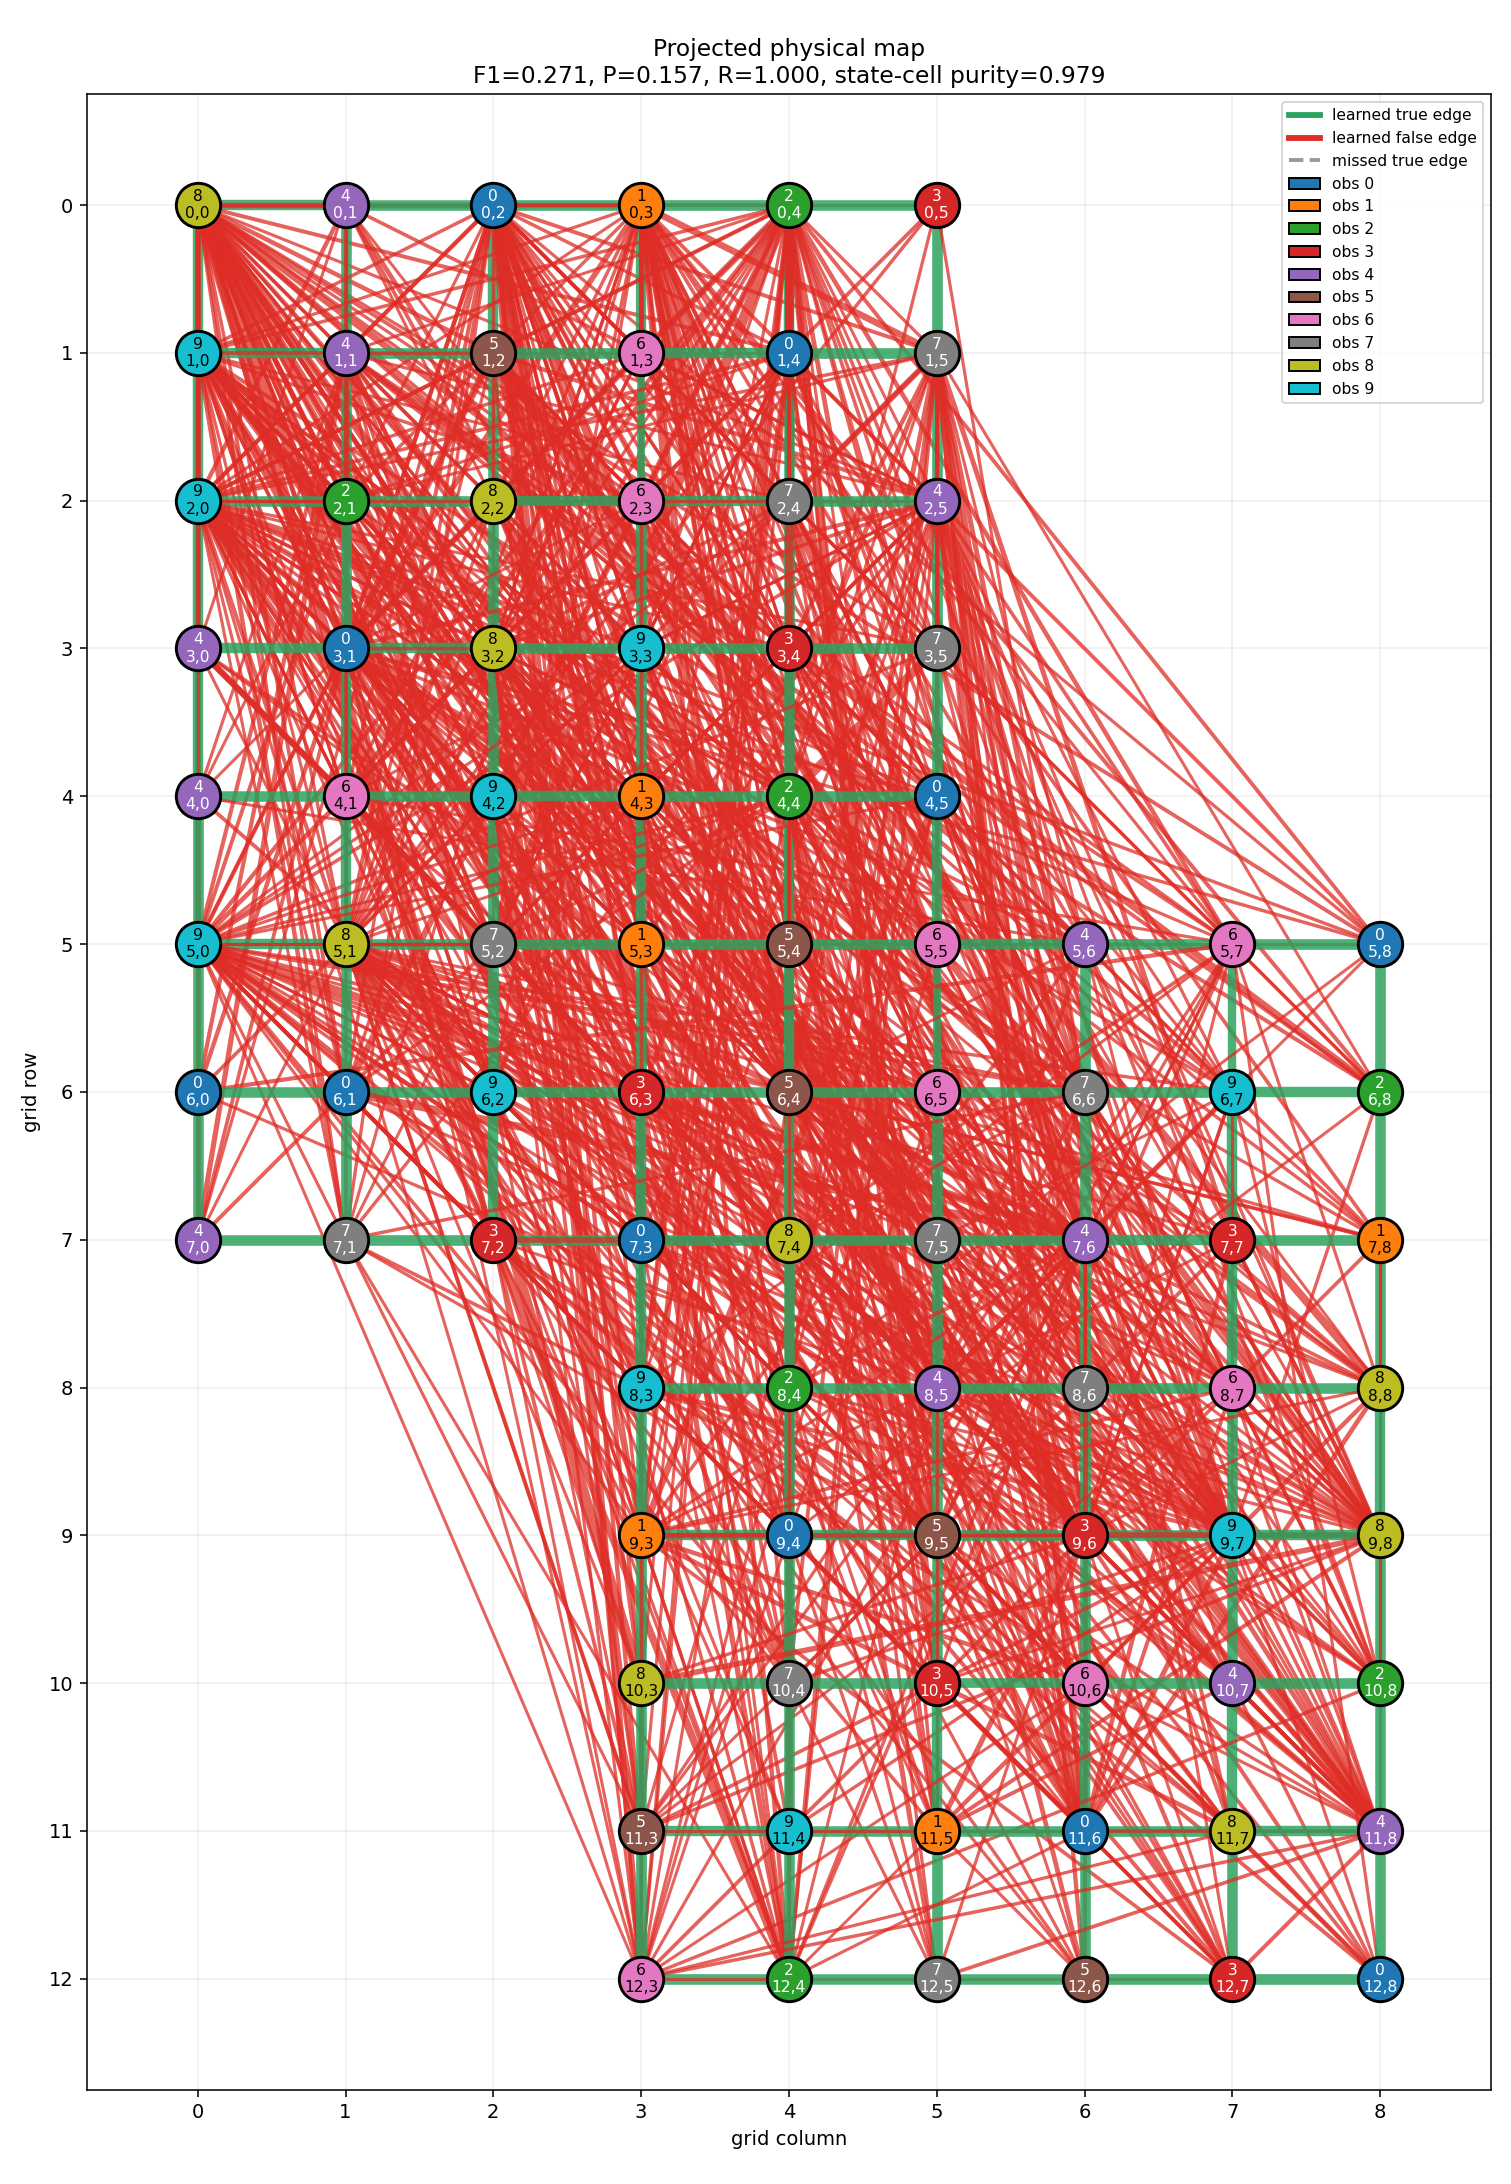
\includegraphics[width=0.72\columnwidth,height=0.44\textheight,%
keepaspectratio]{projected_physical_graph.png}
\caption{Learned map for \texttt{two\_rooms} projected onto the true grid.
Green: correctly recovered edges; red: false edges; grey dashed: missed edges
(none). Node colour encodes the observation digit.}
\label{fig:projected}
\end{figure}

\subsection{Cross-environment summary}
Table~\ref{tab:results} collects all results. The pipeline succeeds on every
environment, including the largest (\texttt{two\_rooms}, $13\times9$): clone
purity $0.83$--$0.90$, state-to-place purity $0.95$--$0.98$, action-outcome
accuracy $0.94$--$1.00$, recall $1.00$, and best-threshold map F1
$0.67$--$0.87$.

\begin{table*}[t]
\centering
\caption{Main results. All runs use the full Phase~2 $\to$ finalization
pipeline. ``State$\to$place purity'' is visit-weighted. ``Recall'' and ``Best
F1'' are map-edge metrics; recall is reported at $\eta=0.01$ and best F1 over
the sweep of Table~\ref{tab:sweep}. The \texttt{aliased} run predates the
map-recovery suite ($\dagger$); it is the cleanest perception case (exactly one
token per cell, perplexity $=K$).}
\label{tab:results}
\small
\resizebox{\textwidth}{!}{%
\begin{tabular}{@{}lccccccccc@{}}
\toprule
\textbf{Environment} & \textbf{Grid} & \textbf{$K$} & \textbf{$N$} &
\textbf{Perplexity} & \textbf{Clone purity} &
\textbf{State$\to$place purity} & \textbf{Action acc.} &
\textbf{Map recall} & \textbf{Best map F1}\\
\midrule
\texttt{aliased}        & $4\times4$  & $4$  & $21$  & $4.00$ & $0.84$ & ---$^\dagger$ & ---$^\dagger$ & ---$^\dagger$ & ---$^\dagger$\\
\texttt{corridors}      & $5\times5$  & $6$  & $31$  & $5.71$ & $0.86$ & $0.98$ & $\mathbf{1.00}$ & $1.00$ & $\mathbf{0.87}$\\
\texttt{room} (uniform) & $6\times6$  & $10$ & $201$ & $6.63$ & $\mathbf{0.90}$ & $0.98$ & $0.94$ & $1.00$ & $0.67$\\
\texttt{room} (dynamic) & $6\times6$  & $10$ & $57$  & $6.56$ & $0.83$ & $0.95$ & $0.97$ & $1.00$ & $0.85$\\
\texttt{two\_rooms}     & $13\times9$ & $10$ & $151$ & $9.46$ & $0.88$ & $0.98$ & $0.99$ & $1.00$ & $0.86$\\
\bottomrule
\end{tabular}}
\end{table*}

\subsection{Training dynamics}
Figure~\ref{fig:loss} shows the loss trajectories. Reconstruction is stable
across joint training; the length-normalized HMM term decreases steadily once
$\lambda_t$ ramps in; and the finalization phase produces a further sharp drop
in HMM NLL with the encoder frozen --- consistent with the role of the
balancing terms in Section~\ref{sec:joint}.

\begin{figure*}[t]
\centering
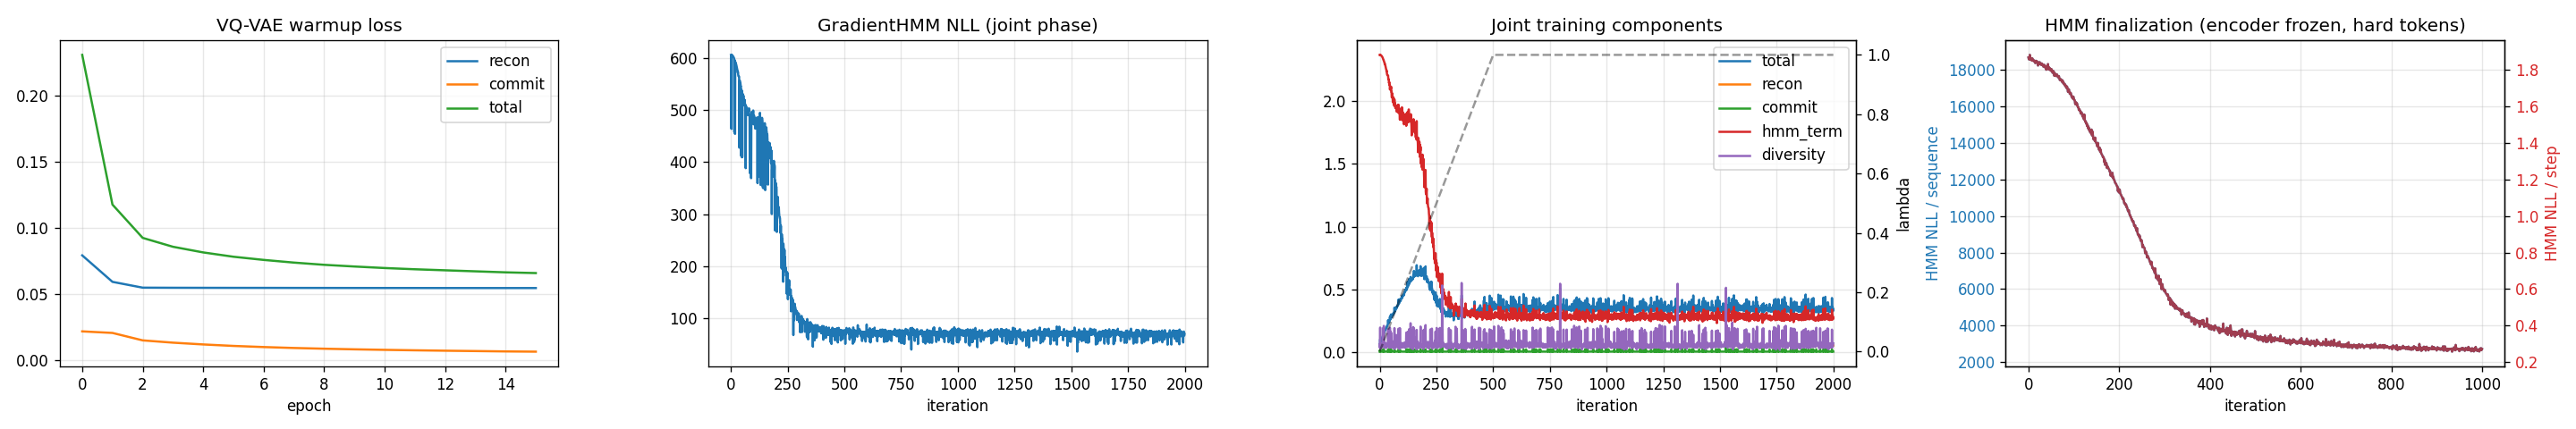
\includegraphics[width=0.96\textwidth]{loss_curves.png}
\caption{Training curves for \texttt{two\_rooms}: VQ-VAE warmup, joint-phase
components (reconstruction, commitment, length-normalized HMM term,
diversity), and the pure-HMM finalization phase.}
\label{fig:loss}
\end{figure*}

% ---------------------------------------------------------------------
\section{Discussion}
\label{sec:discussion}

The experiments support the paper's central claim: topology recovery emerges
from the \emph{interaction} of the two modules, not from either alone.
Perception must discretize finely enough for sequence learning; the cloned HMM
must use action context to disambiguate aliasing; and the resulting latent
graph must align with physical adjacency. Empirically, the encoder converges
to roughly one token per place ($H(\text{token}\mid\text{place})\le0.23$
nats), the clones absorb the aliasing (state-to-place purity $\ge0.95$), and
the learned graph contains the entire true map (recall $1.00$). The
soft-emission coupling (Section~\ref{sec:soft}) is the mechanism that lets the
topological objective influence perception, and the loss-balancing terms
(Section~\ref{sec:joint}) are what make that coupling trainable: without length
normalization and the diversity penalty, joint training collapses the codebook.

% ---------------------------------------------------------------------
\section{Limitations}
\label{sec:limitations}

Three limitations should be stated plainly. \emph{(i) Precision.} The learned
graph recovers every true edge but also adds weak false edges; high F1
currently depends on selecting an edge threshold. Threshold-free sharpening
--- stronger transition-entropy regularization, edge calibration --- is the
immediate next step. \emph{(ii) Scope.} Results are on a controlled MNIST
grid-world; a 3-D, image-based environment is future work. \emph{(iii)
Supervision.} A benchmark-only digit-classification loss is available for the
VQ-VAE warmup; the long-term claim must rest on the fully unsupervised
front-end, which the framework supports but which we have not exhaustively
characterized here.

% ---------------------------------------------------------------------
\section{Conclusion}
\label{sec:conclusion}

We presented neuralCSCG, an end-to-end pipeline that learns the topological
cognitive map of an environment directly from streams of images and actions.
The technical core is a differentiable, soft-emission cloned HMM whose forward
algorithm propagates gradients into a VQ-VAE perceptual front-end, together
with loss-balancing mechanisms that make joint training stable. On five MNIST
grid-world environments with strong perceptual aliasing the method recovers
the physical adjacency graph with perfect edge recall, high state-to-place
purity, and best-threshold map F1 of $0.67$--$0.87$. The remaining frontier is
edge precision and the move to richer, three-dimensional environments.

\paragraph{Code and data availability.}
The implementation, benchmark environments, training scripts and evaluation
suite are available in the project repository.

% ---------------------------------------------------------------------
\begin{thebibliography}{9}
\small

\bibitem{tolman1948}
E.~C. Tolman.
\newblock Cognitive maps in rats and men.
\newblock \emph{Psychological Review}, 55(4):189--208, 1948.

\bibitem{george2021}
D.~George, R.~V. Rikhye, N.~Gothoskar, J.~S. Guntupalli, A.~Dedieu, and
  M.~L\'azaro-Gredilla.
\newblock Clone-structured graph representations enable flexible learning and
  vicarious evaluation of cognitive maps.
\newblock \emph{Nature Communications}, 12:2392, 2021.

\bibitem{whittington2020}
J.~C.~R. Whittington, T.~H. Muller, S.~Mark, G.~Chen, C.~Barry, N.~Burgess, and
  T.~E.~J. Behrens.
\newblock The Tolman--Eichenbaum Machine: unifying space and relational memory
  through generalization in the hippocampal formation.
\newblock \emph{Cell}, 183(5):1249--1263, 2020.

\bibitem{oord2017}
A.~van~den Oord, O.~Vinyals, and K.~Kavukcuoglu.
\newblock Neural discrete representation learning.
\newblock In \emph{Advances in Neural Information Processing Systems (NeurIPS)},
  2017.

\bibitem{razavi2019}
A.~Razavi, A.~van~den Oord, and O.~Vinyals.
\newblock Generating diverse high-fidelity images with VQ-VAE-2.
\newblock In \emph{Advances in Neural Information Processing Systems (NeurIPS)},
  2019.

\bibitem{bengio2013}
Y.~Bengio, N.~L\'eonard, and A.~Courville.
\newblock Estimating or propagating gradients through stochastic neurons for
  conditional computation.
\newblock \emph{arXiv:1308.3432}, 2013.

\bibitem{rabiner1989}
L.~R. Rabiner.
\newblock A tutorial on hidden Markov models and selected applications in speech
  recognition.
\newblock \emph{Proceedings of the IEEE}, 77(2):257--286, 1989.

\bibitem{kingma2015}
D.~P. Kingma and J.~Ba.
\newblock Adam: a method for stochastic optimization.
\newblock In \emph{International Conference on Learning Representations (ICLR)},
  2015.

\bibitem{lecun1998}
Y.~LeCun, L.~Bottou, Y.~Bengio, and P.~Haffner.
\newblock Gradient-based learning applied to document recognition.
\newblock \emph{Proceedings of the IEEE}, 86(11):2278--2324, 1998.

\end{thebibliography}

\end{document}
